\chapter{針對不同使用情境進行最佳化}
\label{chp:5}

\begin{figure}[htpb]
    \centering
    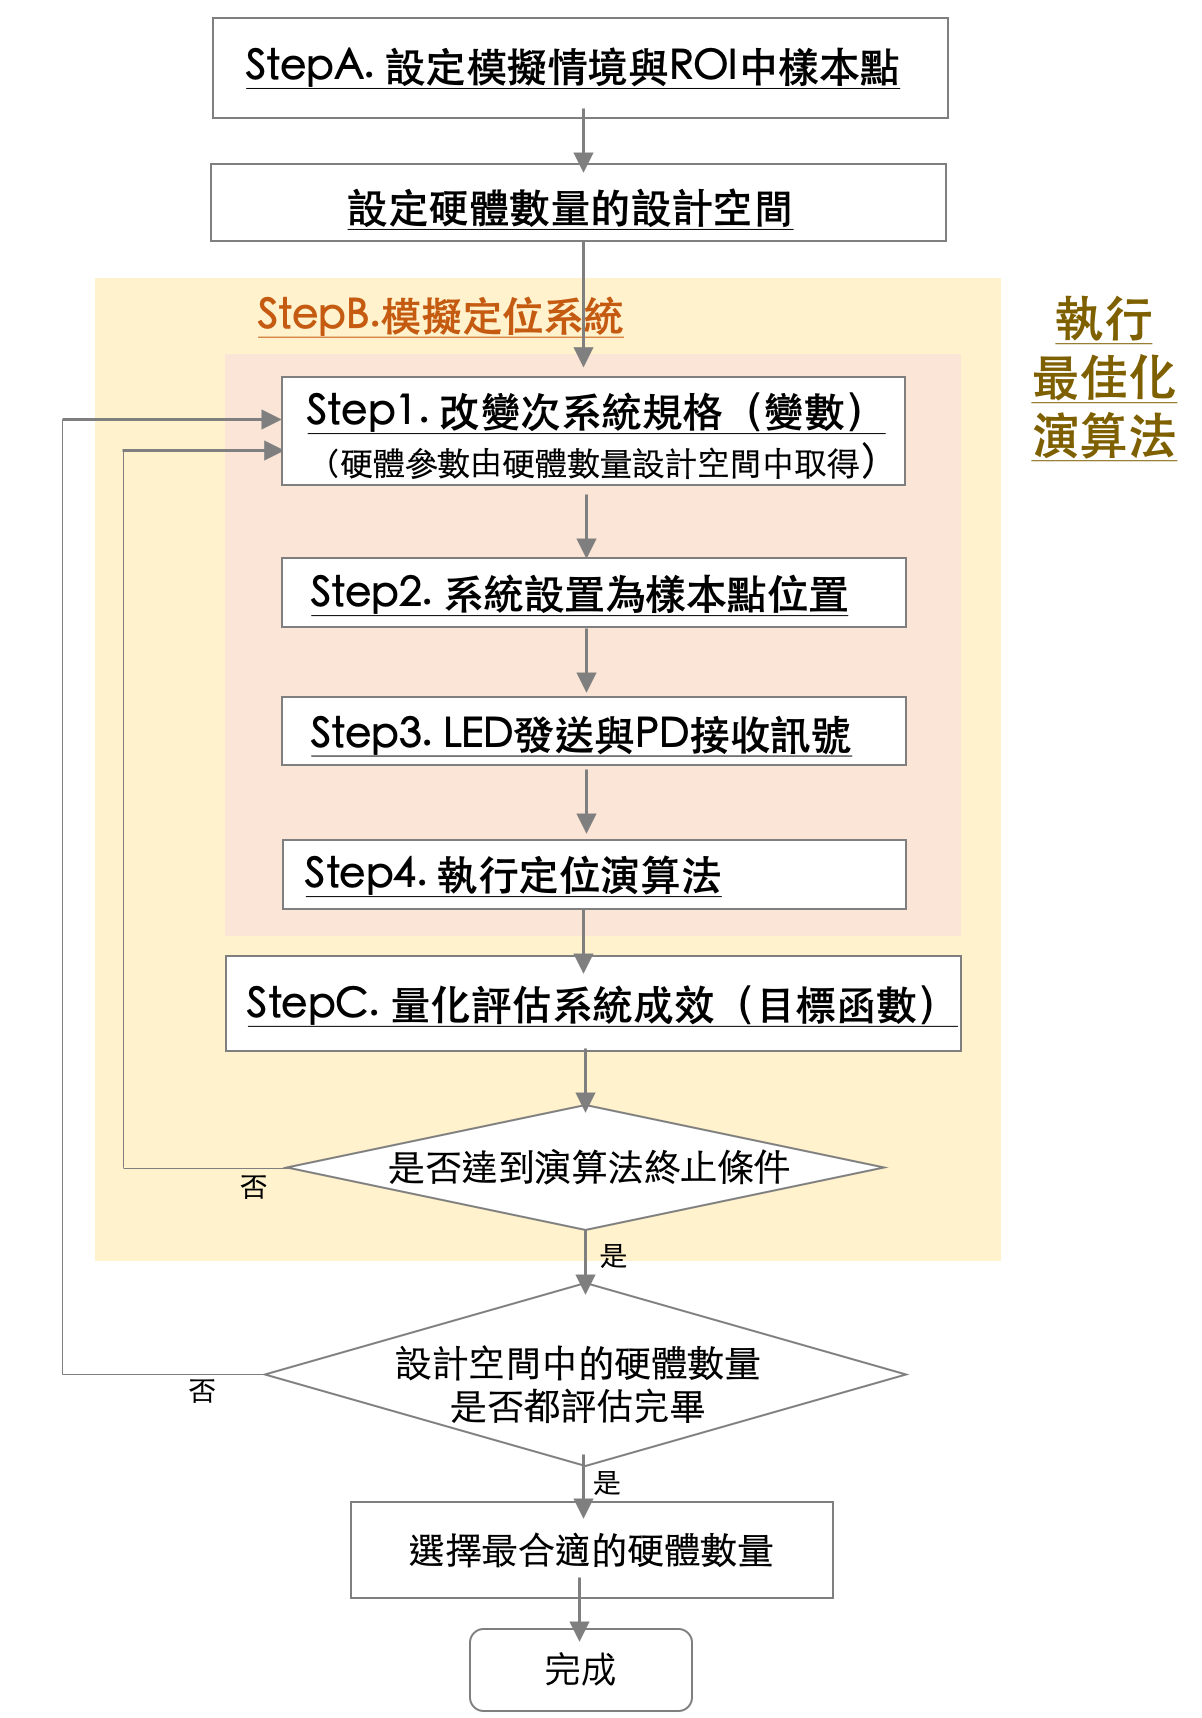
\includegraphics[width=11cm]{ch5pic/optimize_flow.png}
    \caption{最佳化流程圖}
    \label{pic:optimize_flow}
\end{figure}

我們於第四章中,討論了不同次系統規格的變數對硬體成效的影響,然而在第四章中為了方便分析,我們限制硬體指向使變數只剩下LED與PD的硬體天頂角;在分析上,各參數的影響也僅透過固定其他參數來作分析。因此,當我們想要針對特定使用情境,得到最好的次系統規格,則需要透過最佳化問題來解答。本章節於依序於\ref{chp:optimize}章定義最佳化問題,並於章中針對\ref{chp:scenario}章中室內定位的例子,於\ref{chp:optimize_case}章給出最佳系統設計,最後於\ref{chp:5_conclu}中進行總結。




因此,本章節的最佳化問題中,最佳化變數包含Step1.決定次系統規格中的:朗博次方$Mp,M\ell$、各硬體指向$^{P}\boldsymbol{V}_p,^{L}\boldsymbol{V}_l$與硬體數量$P,L$,而其中每個硬體皆有硬體指向需要定義,LED在指向總共會有$2L$個自由度、PD則有$2P$個指向自由度。因此最佳化變數的變數總量,又會根據最佳化本身而改變,使得最佳化難度高。因此,為了簡化這個變數數量與變數本身相關的問題,我們將硬體數量獨立出來迭代執行評估,參考流程圖\ref{pic:optimize_flow},與系統評估流程圖\ref{pic:evaluate_flow}相似,由StepA.設定使用情境與ROI中樣本點開始,再設定LED與PD硬體數量的設計空間,接著於StepB.中決定次系統規格並以模擬呈現系統定位流程,最後於StepC.量化系統成效。其中,針對朗博次方與指向的最佳化問題,我們使用基因演算法(Genetic Algorithm,以下簡稱GA)求解,得到該硬體總數$L$與$P$的系統規格中,朗博次方與指向的最佳解後,透過迭代改變硬體數量,最後再人為評估最合適的硬體數量,作為系統最佳解。

% 硬體數量確定後,而,我們可以得到不同硬體數量對應的最佳設計,以及該設計的目標函數。擁有這些資訊,即可透過人類決策者介入選擇,在系統表現以及硬體成本中進行取捨。

% 最佳化流程可藉由對系統評估流程圖\ref{pic:evaluate_flow}修改,呈現於圖\ref{pic:optimize_flow}中。

% 流程其中StepB.中的Step1.決定次系統規格,即為最佳化變數,而StepC.量化系統成效則為目標函數。與系統評估流程差異最大的部分為StepA.與StepB.之間出現的設定硬體數量設計空間,並透過迭代對硬體數量設計空間中的每個設計點進行其他次系統規格參數的最佳化。將硬體數量獨立出來的原因是為了避免最佳化問題過於複雜,詳細可參考\ref{chp:optimize_variable}章。

% 接著與系統評估流程不同,我們將


以下章節依序由\ref{chp:objective}章中介紹目標函數,於\ref{chp:optimize_variable}章中介紹最佳化變數,而\ref{chp:optimize_case}章中則針對情境進行系統最佳化。

\section{最佳化問題}
\label{chp:optimize}
    \subsection{目標函數}
    \label{chp:objective}

    我們的最佳化目標,是希望使系統表現更好,而評估方式可以參考\ref{chp:evaluate_method}章所述的量化標準:容許範圍內的樣本點總數$Nt$,目標是讓此值越高越好,代表著更好的系統成效。因此,在硬體總數設定為$P,L$的情況下,最佳化目標函數$f$呈現於式\ref{eqn:objective}

    \begin{equation}
        \label{eqn:objective}
        \begin{aligned}
        \underset{^{P}\boldsymbol{V}_p, ^{L}\boldsymbol{V}_l,Ml,Mp}{\operatorname{minimize}} 
        \quad f = Nt/K
        \frac{\sum_{i=1}^{K}F(k)}{K}  \\
        \text{Where }F(k)=
        \begin{cases}
            _{k}e<To&,1\\
            else&,0
        \end{cases}
        \end{aligned}
    \end{equation}

    \begin{align*} \text{where }
        &p=1,2,...,P\\&l=1,2,...,L
    \end{align*}


    \subsection{最佳化變數}
    \label{chp:optimize_variable}

    最佳化變數的部分,包含朗博次方$Mp,M\ell$、硬體指向$^{P}\boldsymbol{V}_p,^{L}\boldsymbol{V}_l$與硬體數量$P,L$,而其中每個硬體皆有朗博次方與硬體指向需要定義,因此最佳化的變數量又會根據硬體數量而改變,變數總數為$2+2\times(L+P)$。


    \begin{figure}[htpb]
        \centering
        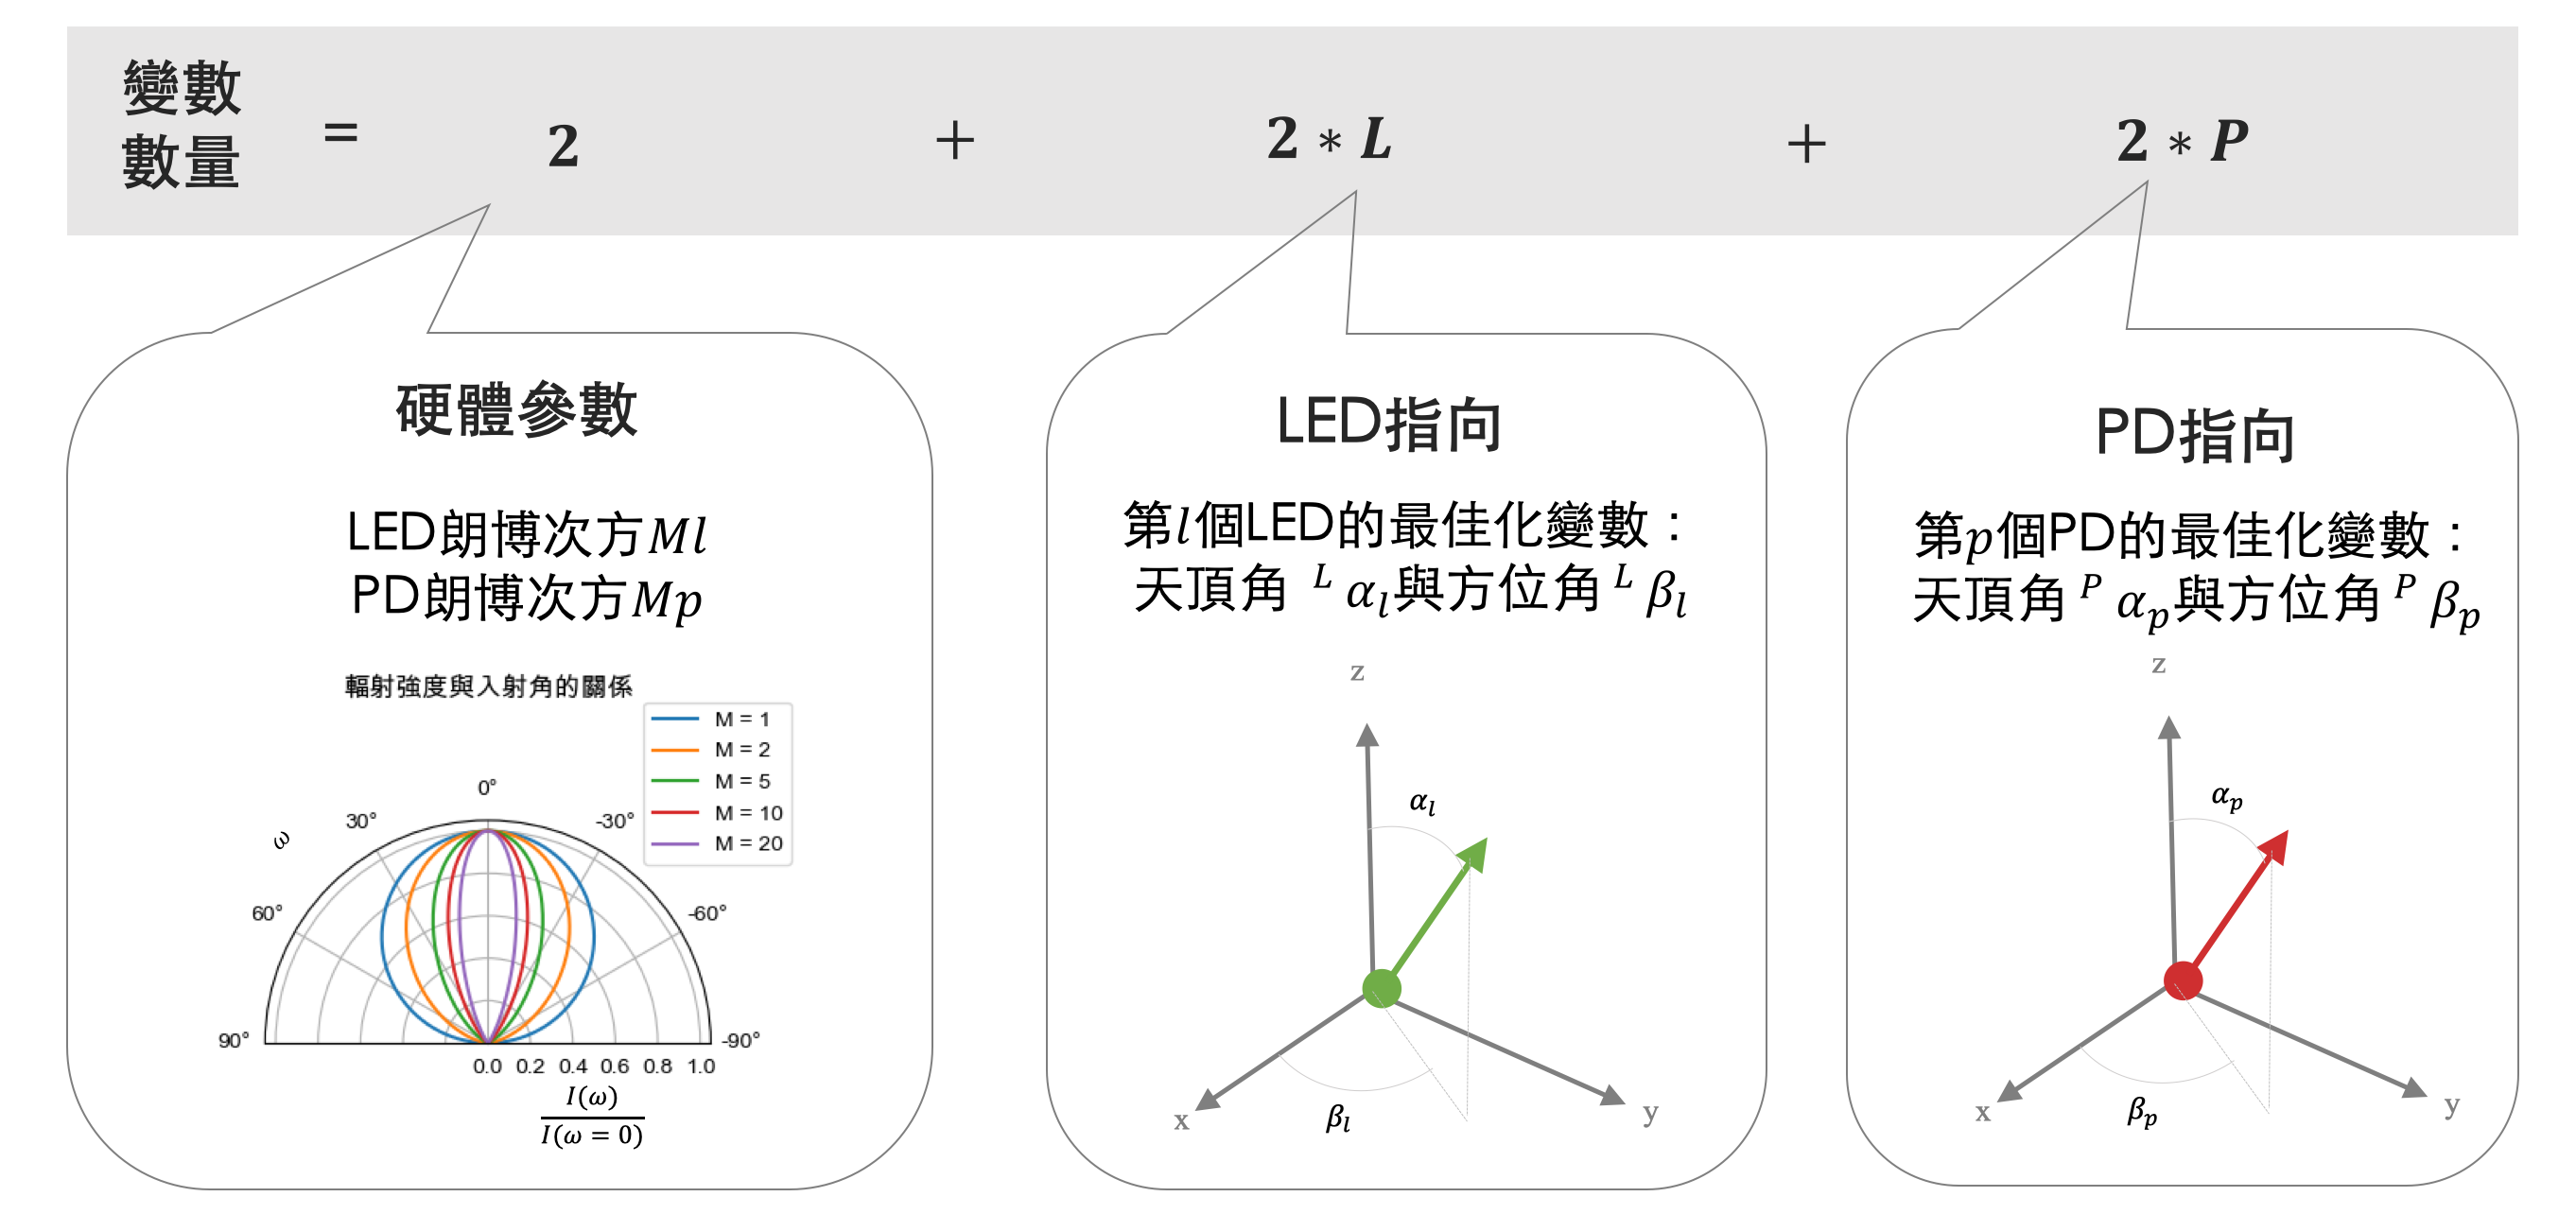
\includegraphics[width=15cm]{ch5pic/optimize_variable.png}
        \caption{最佳化變數}
        \label{pic:optimize_variable}
    \end{figure}



% --------------------------------------
\section{最佳化案例}
\label{chp:optimize_case}

本章節將舉例對不同情境以圖\ref{pic:optimize_flow}中的流程做最佳化,這裡以\ref{chp:scene_effect}章中的使用情境作為例子,其中由於使用情境乙與情境甲僅有範圍差異,因此以下僅對使用情境甲、丙、丁舉例做最佳化,其中使用的誤差模擬參數與除了硬體數量、硬體擺設以及朗博次方以外的硬體參數使用表\ref{tab:para_reference}中的參數。

    \subsection{使用情境甲:$3\times 3\times 3m$空間}
    \label{chp:optimiza_A}

    為針對\ref{chp:scene_A}章中的使用情境進行最佳化,根據圖\ref{pic:optimize_flow}中的流程,我們需先設置硬體數量的設計空間如表\ref{chp:optimiza_A},LED數量由3至8調整而PD數量分別為3、5、8、12。將設計空間中的硬體數量皆以GA進行最佳化,將最佳化回傳之目標函數值呈現於表中,並以圖\ref{pic:opt_A_line}與圖\ref{pic:opt_A_surface}中。由最佳化結果的目標函數值我們可以觀察到增加硬體數量的確能提升系統效能,然而系統效能提升的程度與硬體數量的程度並不符合,隨著硬體數量提升的系統效能會逐漸趨緩,達到一極限。因此,在選擇合適硬體參數時需在系統效能與硬體系統複雜度中做出合理的選擇。於硬體設計空間中選擇出符合預期效能又符合硬體搭建成本與複雜度的選擇。

    % \begin{figure}[htpb]
    %     \centering
    %     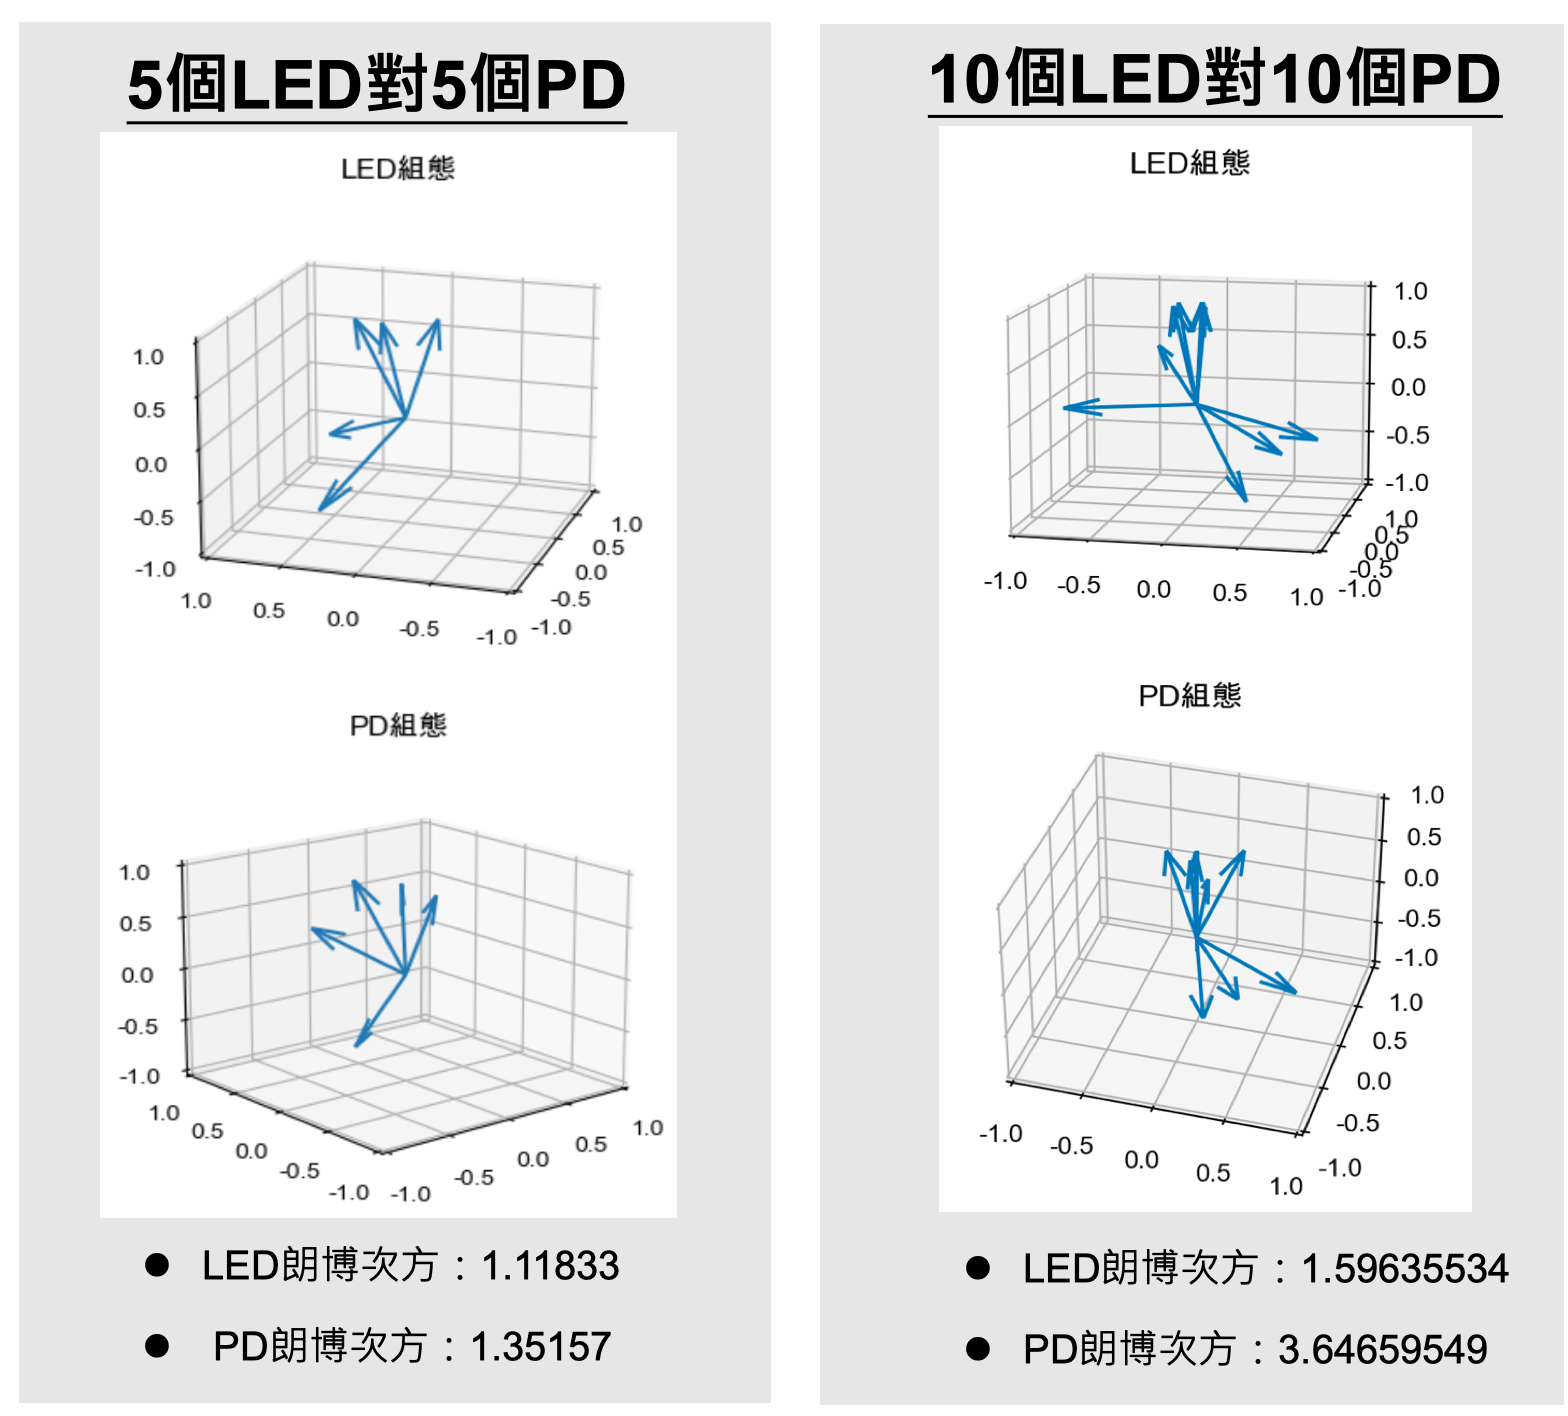
\includegraphics[width=15cm]{ch5pic/opt_result.png}
    %     \caption{最佳化結果}
    %     \label{pic:opt_result}
    % \end{figure}

    % 觀察這兩個系統設計的差別,在硬體數量少的時候,為了讓空間中的最多個樣本點可讀到訊號,因此朗博次方較小,捨棄了對出入射角敏感度。

    \begin{table}[htpb]
        \begin{center}
          \caption{使用情境甲的最佳化後的目標函數值(樣本總數K=61000)}
          \label{tab:optimize_A}
          \begin{tabular}{c||c|c|c|c|c|c} % <-- Alignments: 1st column left, 2nd middle and 3rd right, with vertical lines in between
            \diagbox{PD數量}{LED數量}& 3&4&5&6&7&8\\
            \hline

            3&39522&42216&42828&43765&43777&43265\\
            5&43792&45279&47893&48378&48844&48377\\
            8&47483&48005&52609&53191&53465&54144\\
            12&50511&50677&54010&56550&56272&56685\\
          \end{tabular}
        \end{center}
      \end{table}

    \begin{figure}[htpb]
        \centering
        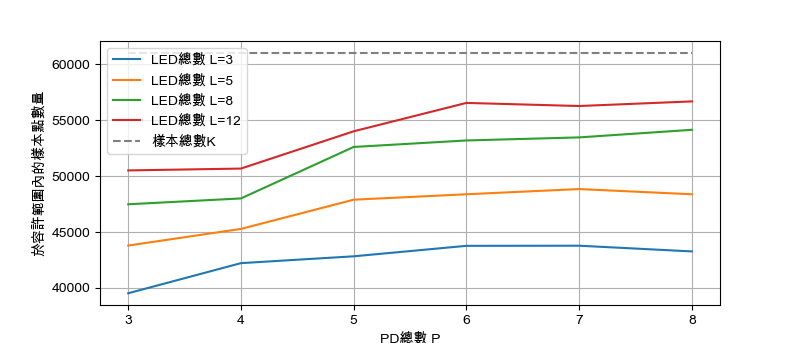
\includegraphics[width=15cm]{ch5pic/optimize_A.png}
        \caption{情境甲的最佳化後的目標函數值}
        \label{pic:opt_A_line}
    \end{figure}

    \begin{figure}[htpb]
        \centering
        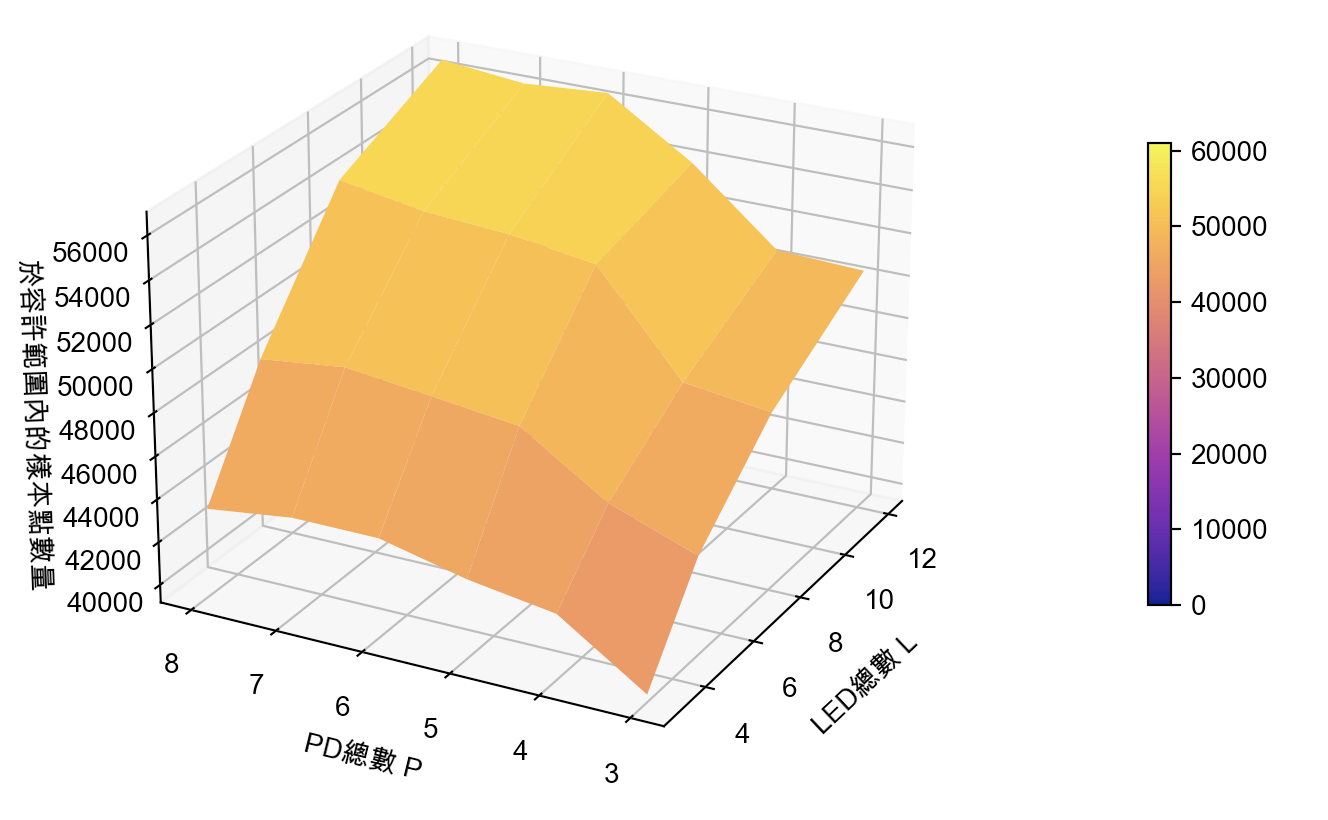
\includegraphics[width=15cm]{ch5pic/surface_opt_A.png}
        \caption{情境甲的最佳化後的目標函數值(以平面呈現)}
        \label{pic:opt_A_surface}
    \end{figure}

    除了最佳化後的目標函數值以外,各硬體數量對應之最佳化變數的最佳解也值得注意,而最佳化變數包含朗博次方與硬體指向。在情境甲的情況中,所有硬體數量設計範圍內的朗博次方最佳解都是非常接近1的數值,也就是在覆蓋範圍與對角度敏感度之間選擇了覆蓋範圍,其表現符合預期,在情境甲同時包含遠近、不同方位與相對姿態的大ROI中,為滿足第三章中提出的演算法求解的要求:需有一同時得到三個以上LED訊號的PD以及一同時傳遞至三個PD的LED硬體才得以求解,在情境甲的狀況中最佳解的朗博次方都非常接近一。至於硬體擺設的最佳解,由於變數多難統一討論,我們舉硬體數量為$L=P=3$與$L=P=8$這兩個例子,將容許範圍內樣本點比例、有效範圍、與硬體擺設樣式呈現於圖\ref{pic:a_33}與圖\ref{pic:a_88}中。

    \begin{figure}[htpb]
        \centering
        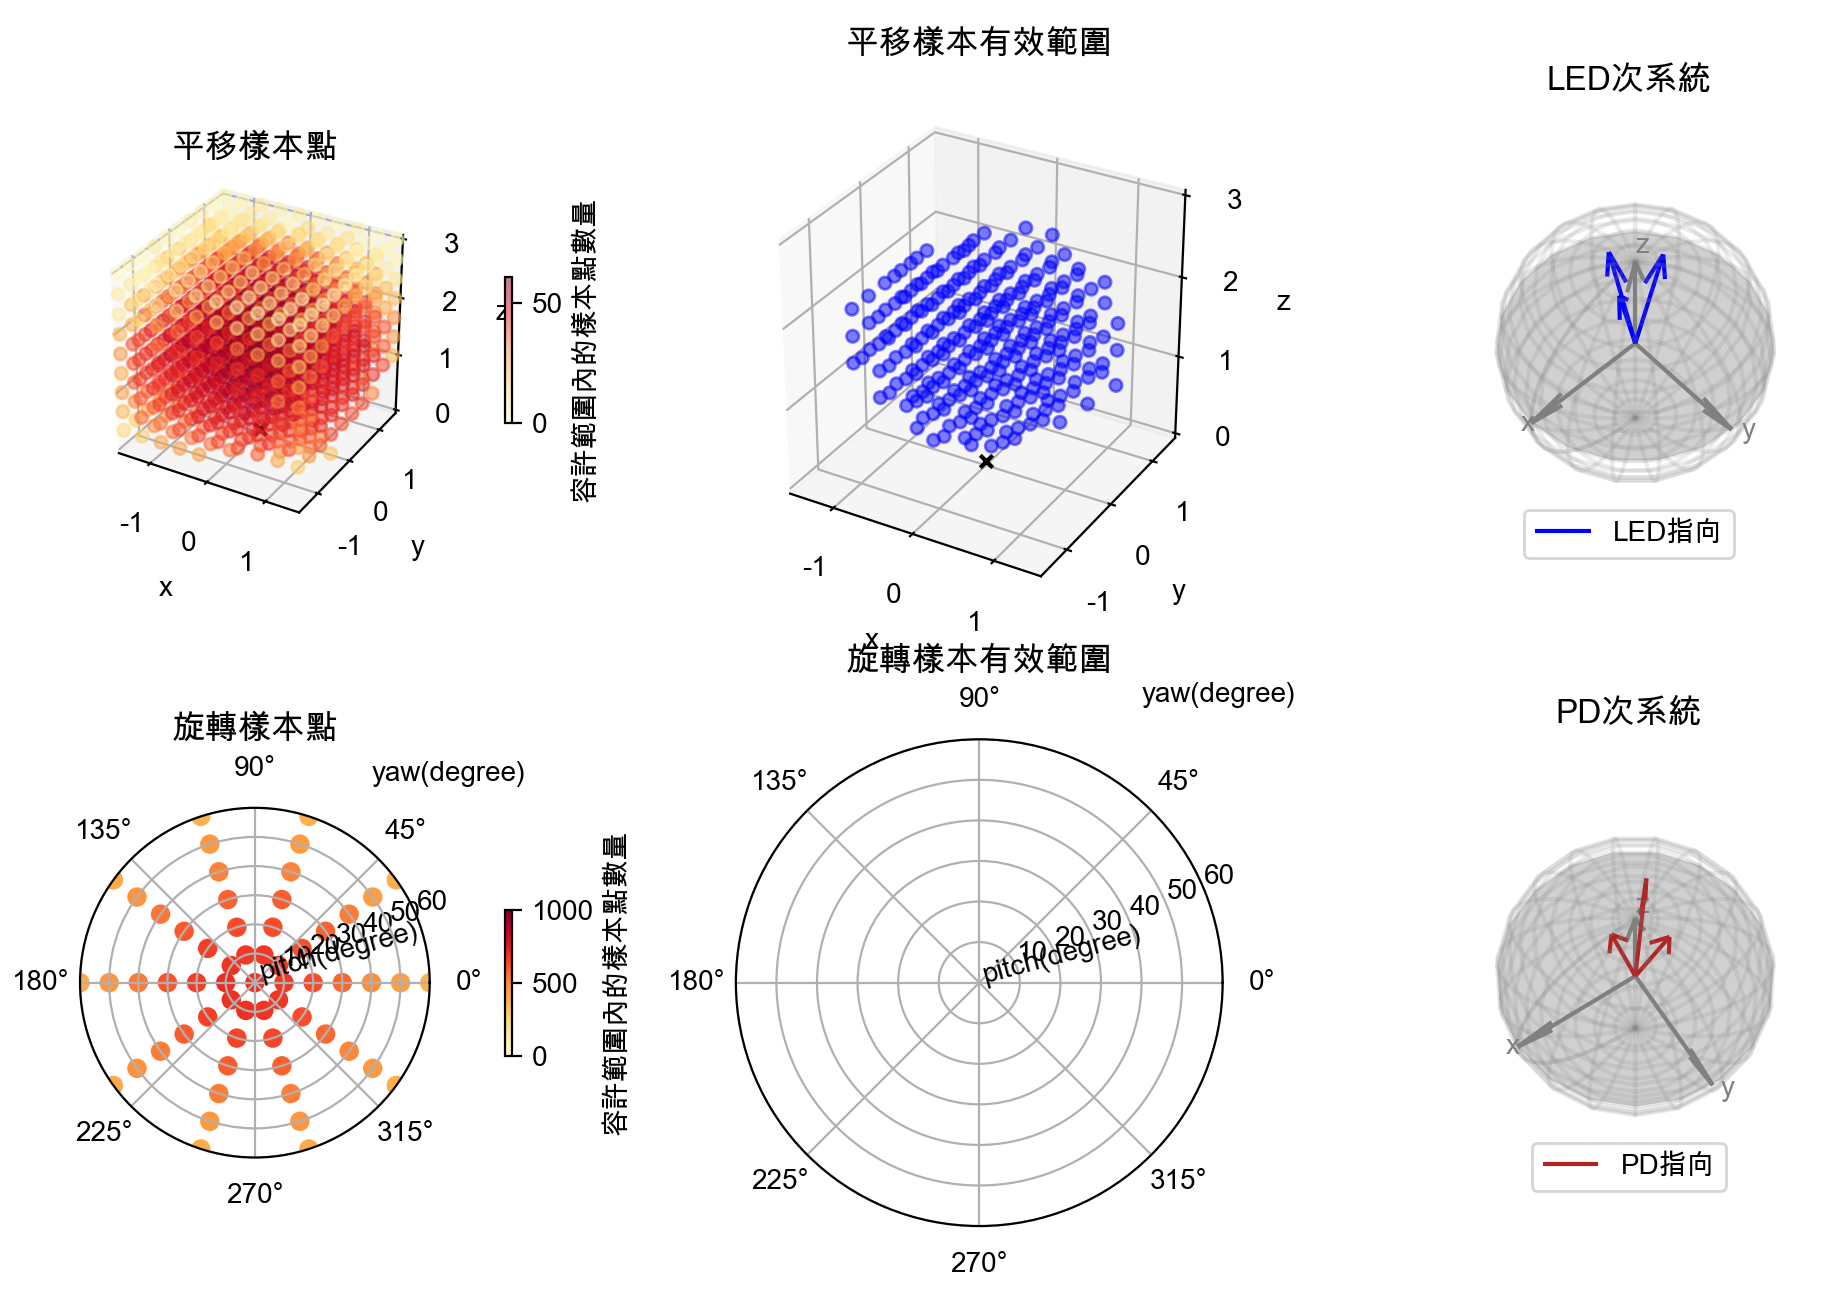
\includegraphics[width=15cm]{ch5pic/a_33.png}
        \caption{情境甲於L=P=3的最佳系統表現與硬體擺設}
        \label{pic:a_33}
    \end{figure}

    \begin{figure}[htpb]
        \centering
        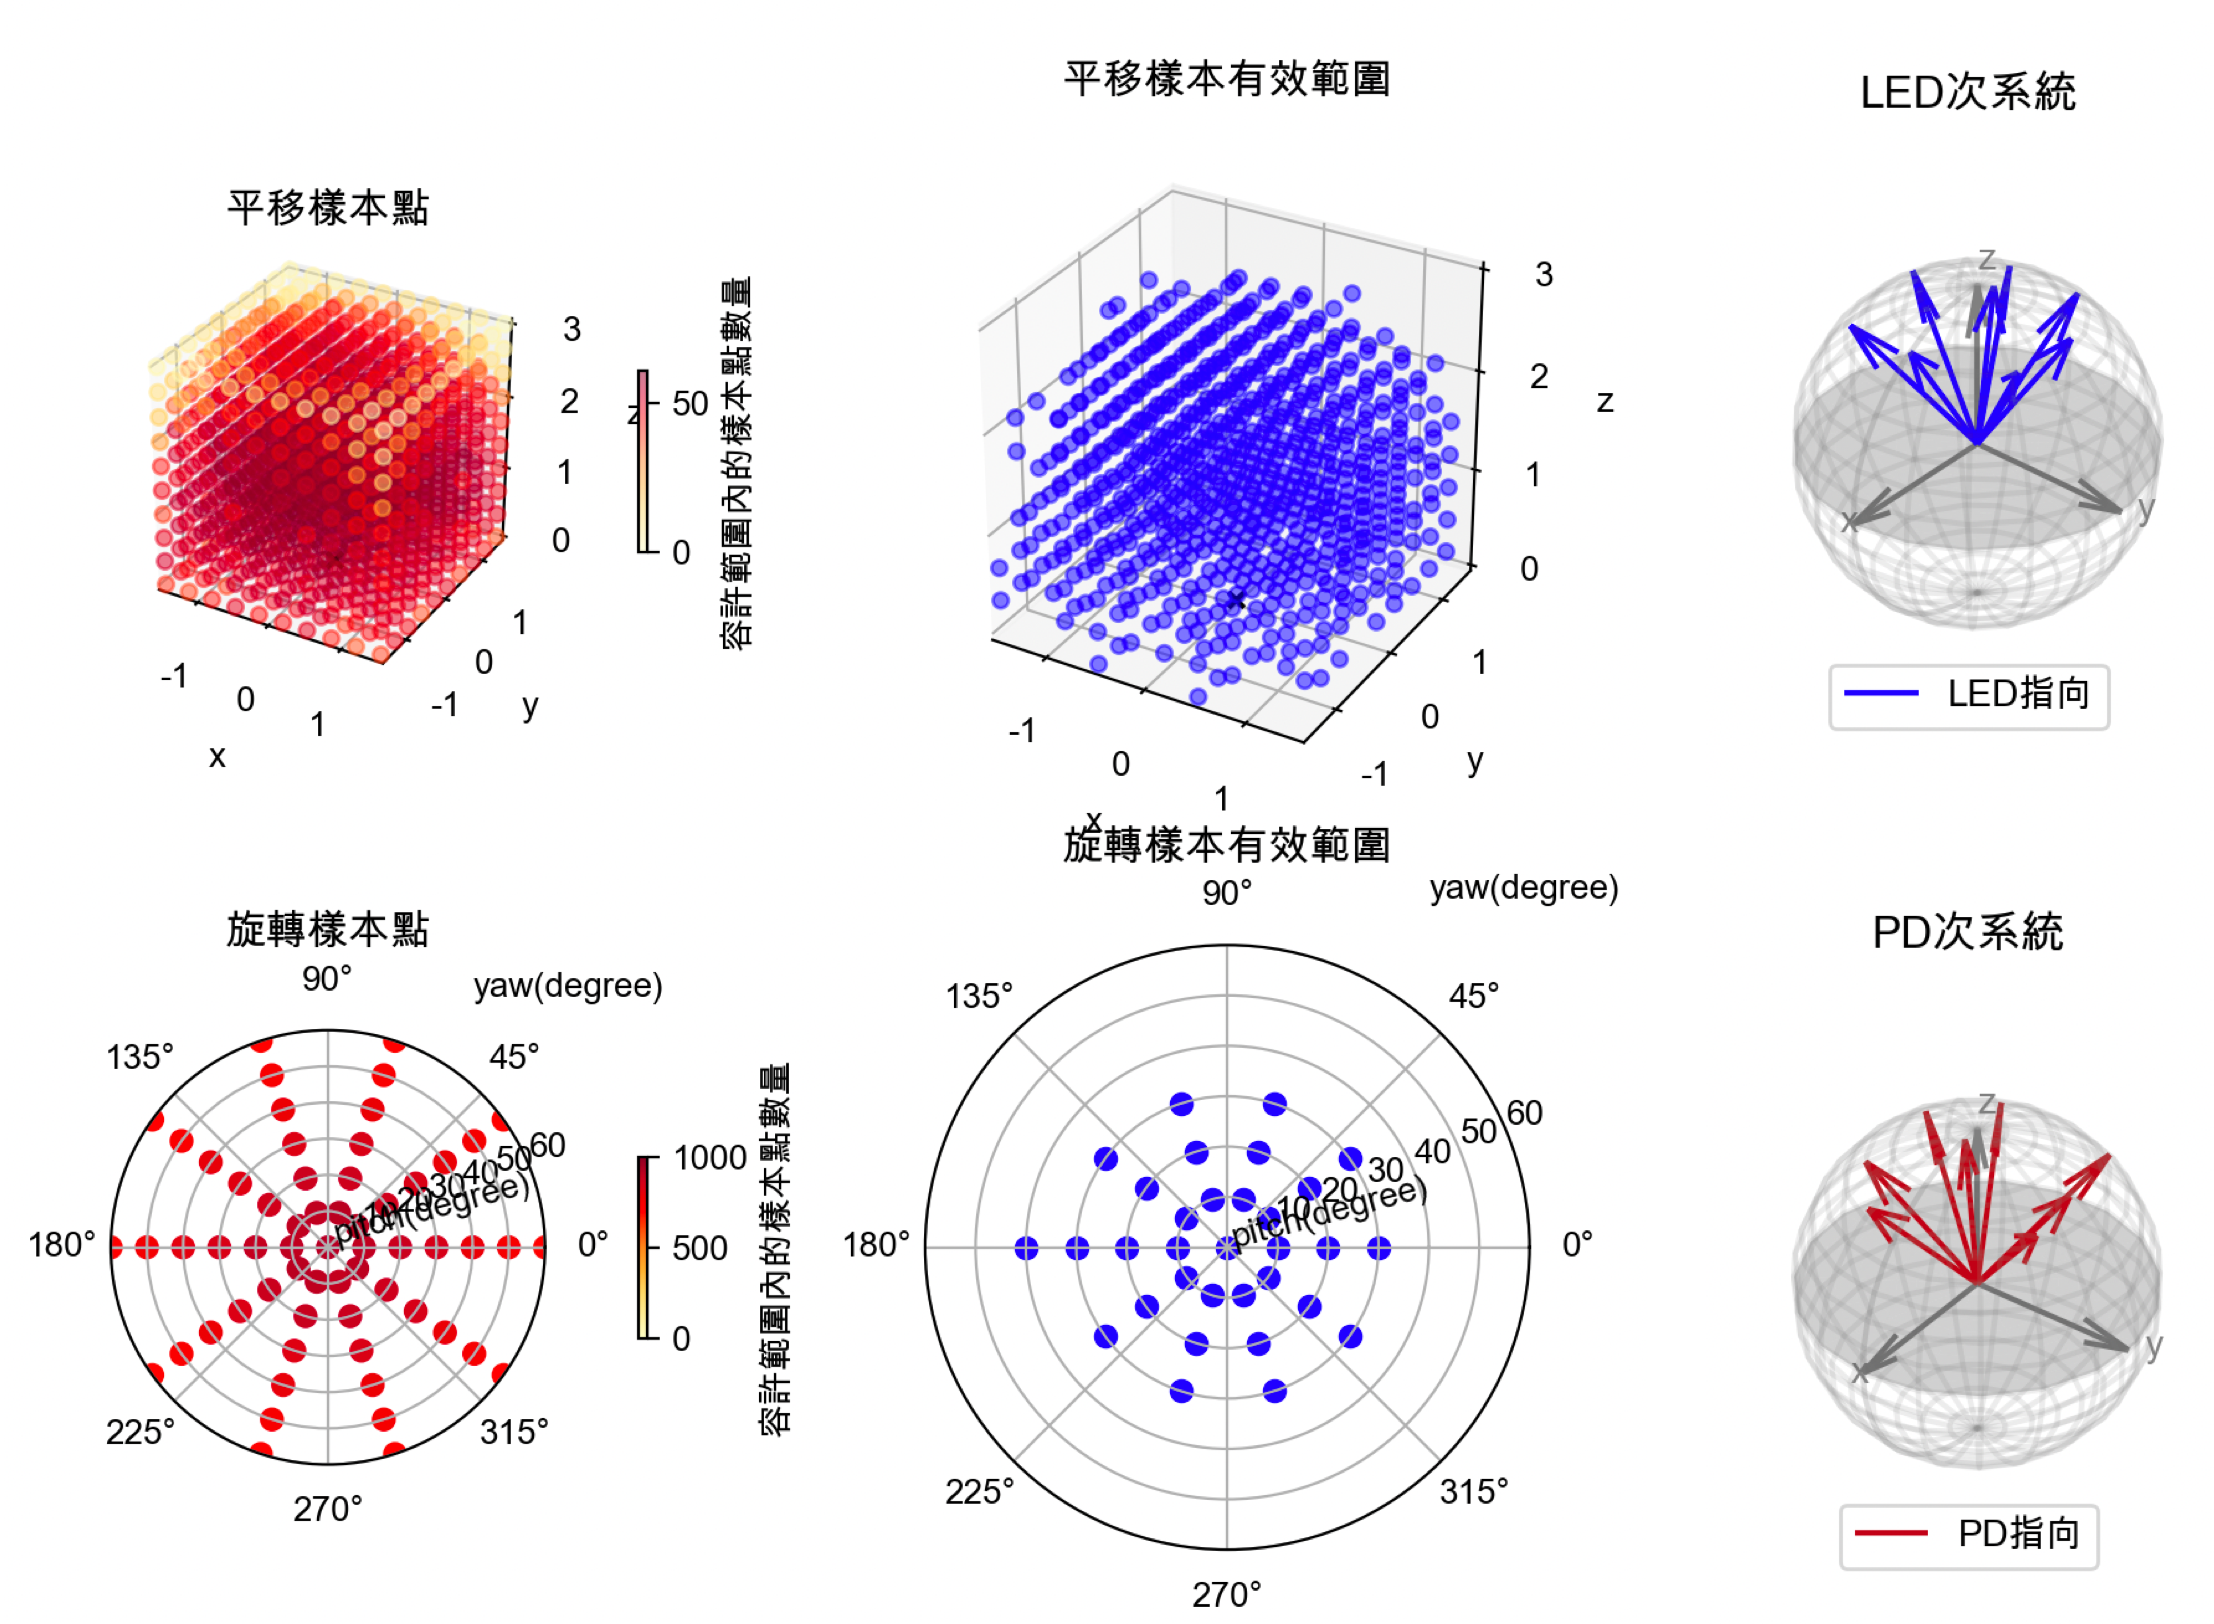
\includegraphics[width=15cm]{ch5pic/a_88.png}
        \caption{情境甲於L=P=8的最佳系統表現與硬體擺設}
        \label{pic:a_88}
    \end{figure}

    圖\ref{pic:a_33}中為了僅用三個硬體解出定位,因此三個硬體之間擺設的角度差異並不大,以使三個硬體的重疊覆蓋範圍增加,滿足第三章Step4.執行定位演算法解出定位的條件。而圖\ref{pic:a_88}的最佳次系統硬體擺設則十分不同,由於硬體數量夠多,呈現各硬體散布於一範圍內。



    % \subsection{以目標物為中心的案例}

    \subsubsection{使用情境丙:平面平行且垂直距離相同}
    \label{chp:optimize_C}

    這邊將硬體設計空間僅考量L=P於數量3至8的範圍,將目標函數的最佳結果呈現於圖\ref{pic:opt_C_line},其中由於使用情境丙的平移樣本點範圍、旋轉樣本點的姿態也僅有平行,在總共$K=10000$個樣本點中,最少的硬體數量$L=P=3$也能達到$100\%$的定位系統成效。因此,容許範圍$To=0.05m$的標準對於此情境來說過於簡單,我們將容許範圍降低至$To=0.03$、$To=0.01$,各自呈現於圖\ref{pic:opt_C_line}中。由圖\ref{pic:opt_C_line}中可觀察到隨著容許範圍下降,樣本點誤差於容許範圍內的總數也隨之下降,而透過提升硬體數量能夠成效$Nt$值。
    
    \begin{figure}[htpb]
        \centering
        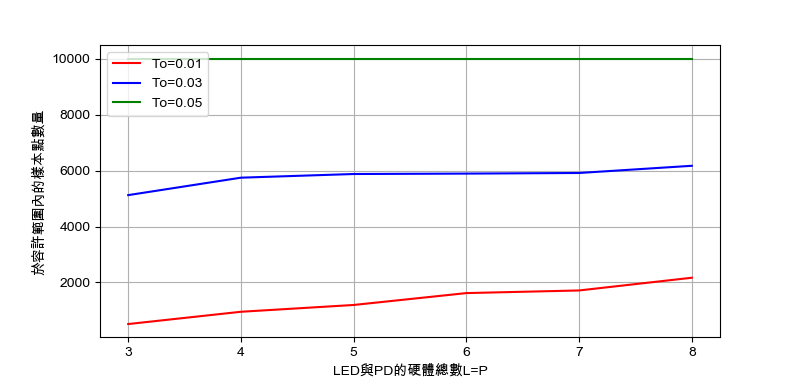
\includegraphics[width=15cm]{ch5pic/optimize_C.png}
        \caption{情境丙的最佳化後的目標函數值}
        \label{pic:opt_C_line}
    \end{figure}

    
    值得注意的是,此情境中的最佳朗博次方解都並非為一,將LED與PD的朗博次方最佳解呈現於表\ref{tab:C_opt_m}中,數值並沒有很明顯的趨勢如圖\ref{pic:c_opt_m},但仍能夠看出於硬體數量較大時最佳朗博次方較大,而容許範圍小的$To=0.01$也有最佳朗博次方較大的趨勢。此趨勢也與預期相同,朗博次方越大代表於角度敏感度與覆蓋範圍中選擇了敏感度,而角度的敏感度能夠幫助精度的提升,因此在容許範圍較小與硬體數量較大時,都選擇了精度犧牲掉部分的覆蓋範圍。

    \begin{table}[htpb]
        \begin{center}
          \caption{使用情境丙最佳朗博次方解}
          \label{tab:C_opt_m}
          \begin{tabular}{c|c||c|c|c|c|c|c} % <-- Alignments: 1st column left, 2nd middle and 3rd right, with vertical lines in between
            容許範圍&LED與PD的硬體數量& 3&4&5&6&7&8\\
            \hline

            \multirow{2}{*}{$To=0.03m$}&LED朗博次方& 1.187&	1.23&	1.24	&1.24&	1.51	&1.5\\
            &PD朗博次方& 1.812&	1.396	&1.5&	1.81&	2.33	&2.385\\\hline
            
            \multirow{2}{*}{$To=0.1m$}&LED朗博次方&
            1.344&	1.5	&1.5&	1.187	&1.292&	1.865\\
            &PD朗博次方&1.656	&2.072	&2.333&	2.177	&2.177&	2.23
          \end{tabular}
        \end{center}
      \end{table}

    \begin{figure}[htpb]
        \centering
        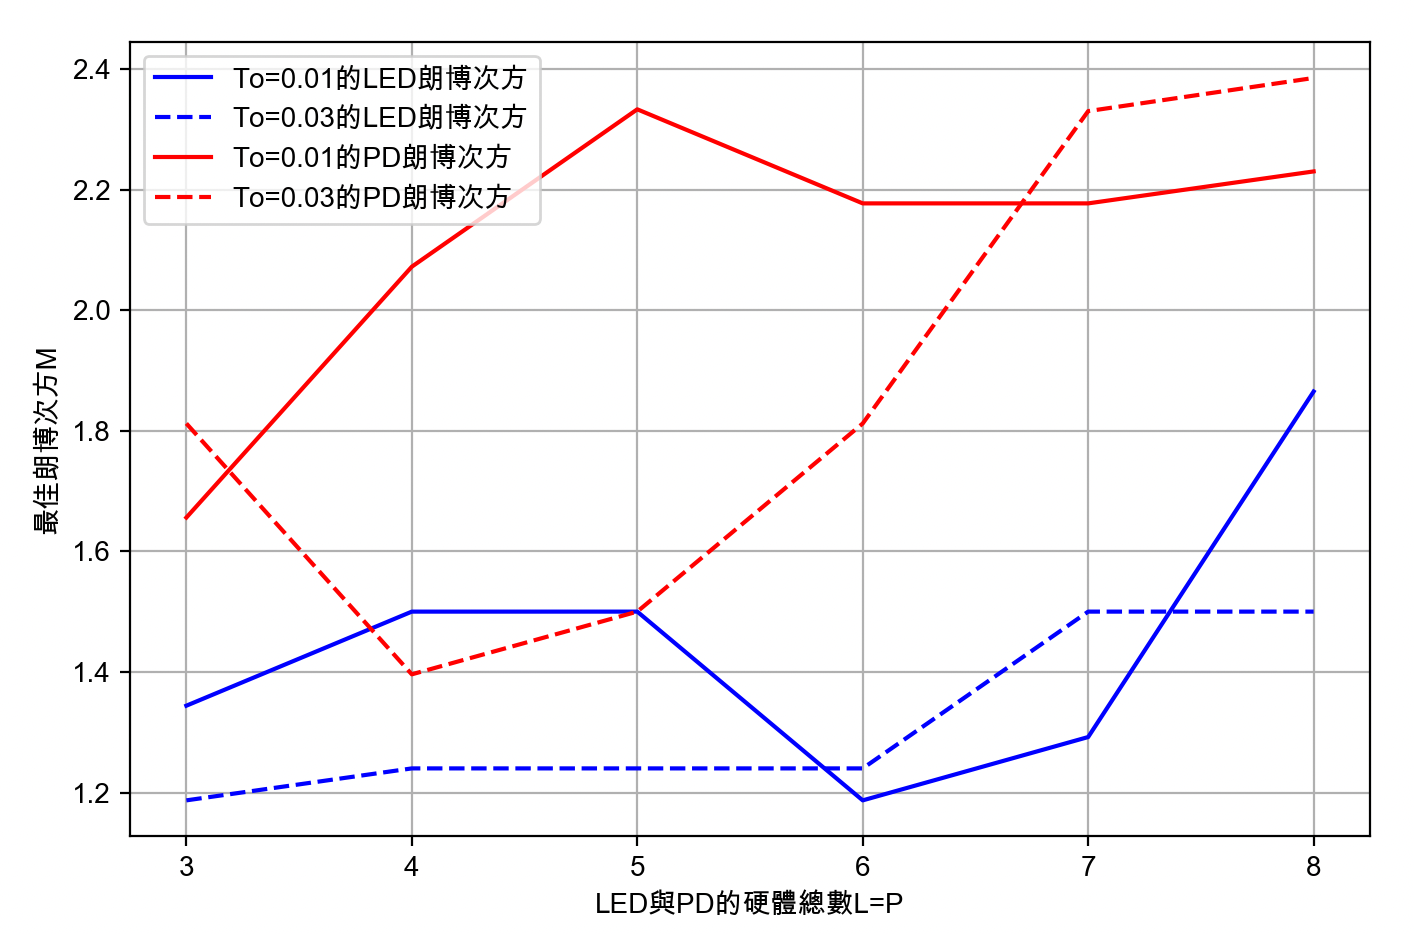
\includegraphics[width=13cm]{ch5pic/c_opt_m.png}
        \caption{情境丙的最佳朗博次方}
        \label{pic:c_opt_m}
    \end{figure}

    


    \subsubsection{使用情境丁:球狀空間}
    \label{chp:optimiza_D}

    這邊一樣考慮硬體設計空間為L=P於數量3至13的範圍,將目標函數的最佳結果呈現於圖\ref{pic:opt_D},同樣隨著硬體數量上升能夠提升系統表現,而在此使用情境中與前兩者不同的是,提升硬體數量由3至8時系統成效提升的非常顯著,所有樣本點於容許範圍內的比例$Nt/K$由$14.4\%$提升至$91.8\%$,於硬體數量大於8之後幅度趨緩。

    \begin{figure}[htpb]
        \centering
        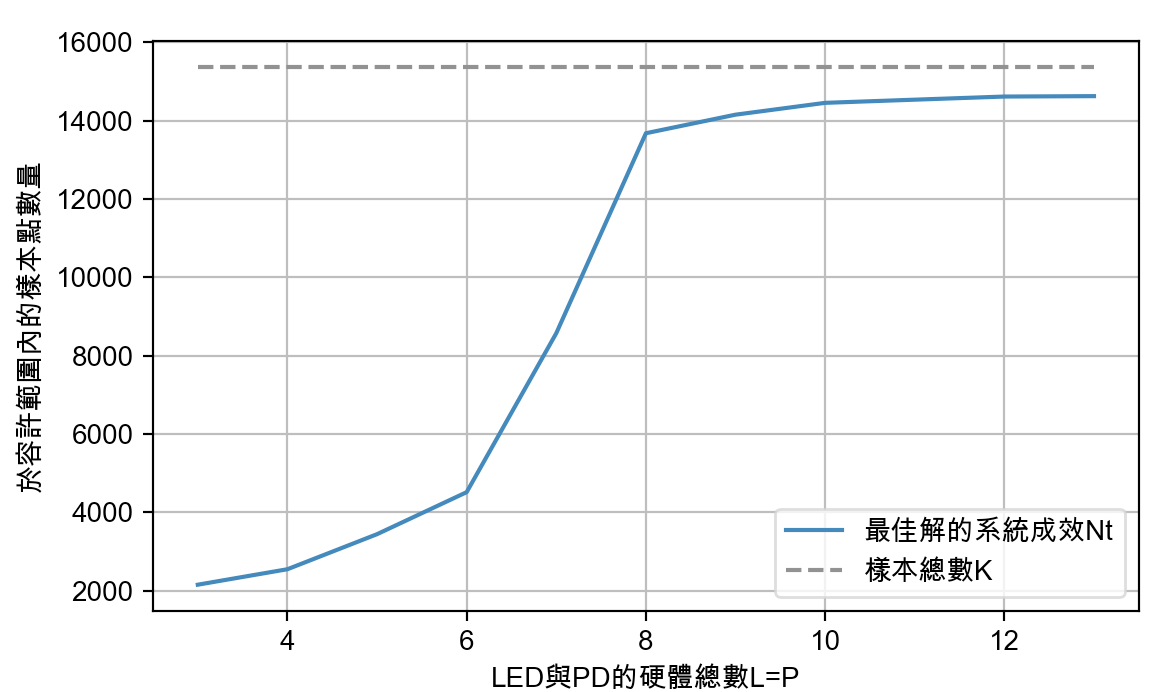
\includegraphics[width=13cm]{ch5pic/optimize_d.png}
        \caption{情境丁的最佳化後的目標函數值}
        \label{pic:opt_D}
    \end{figure}

    最佳朗博次方與情境甲相同,在所有硬體數量中朗博次方都很接近一,凸顯著此使用情境的範圍十分廣。至於最佳硬體擺設方法,我們舉硬體數量$L=P=10$為例呈現於圖\ref{pic:d_1010},在硬體數量$L=P=10$的情況下系統能夠達到$Nt/K=97.1\%$的系統表現,代表在此情境中LED與PD能夠任意旋轉且基本上都能定位於容許範圍內。

    \begin{figure}[htpb]
        \centering
        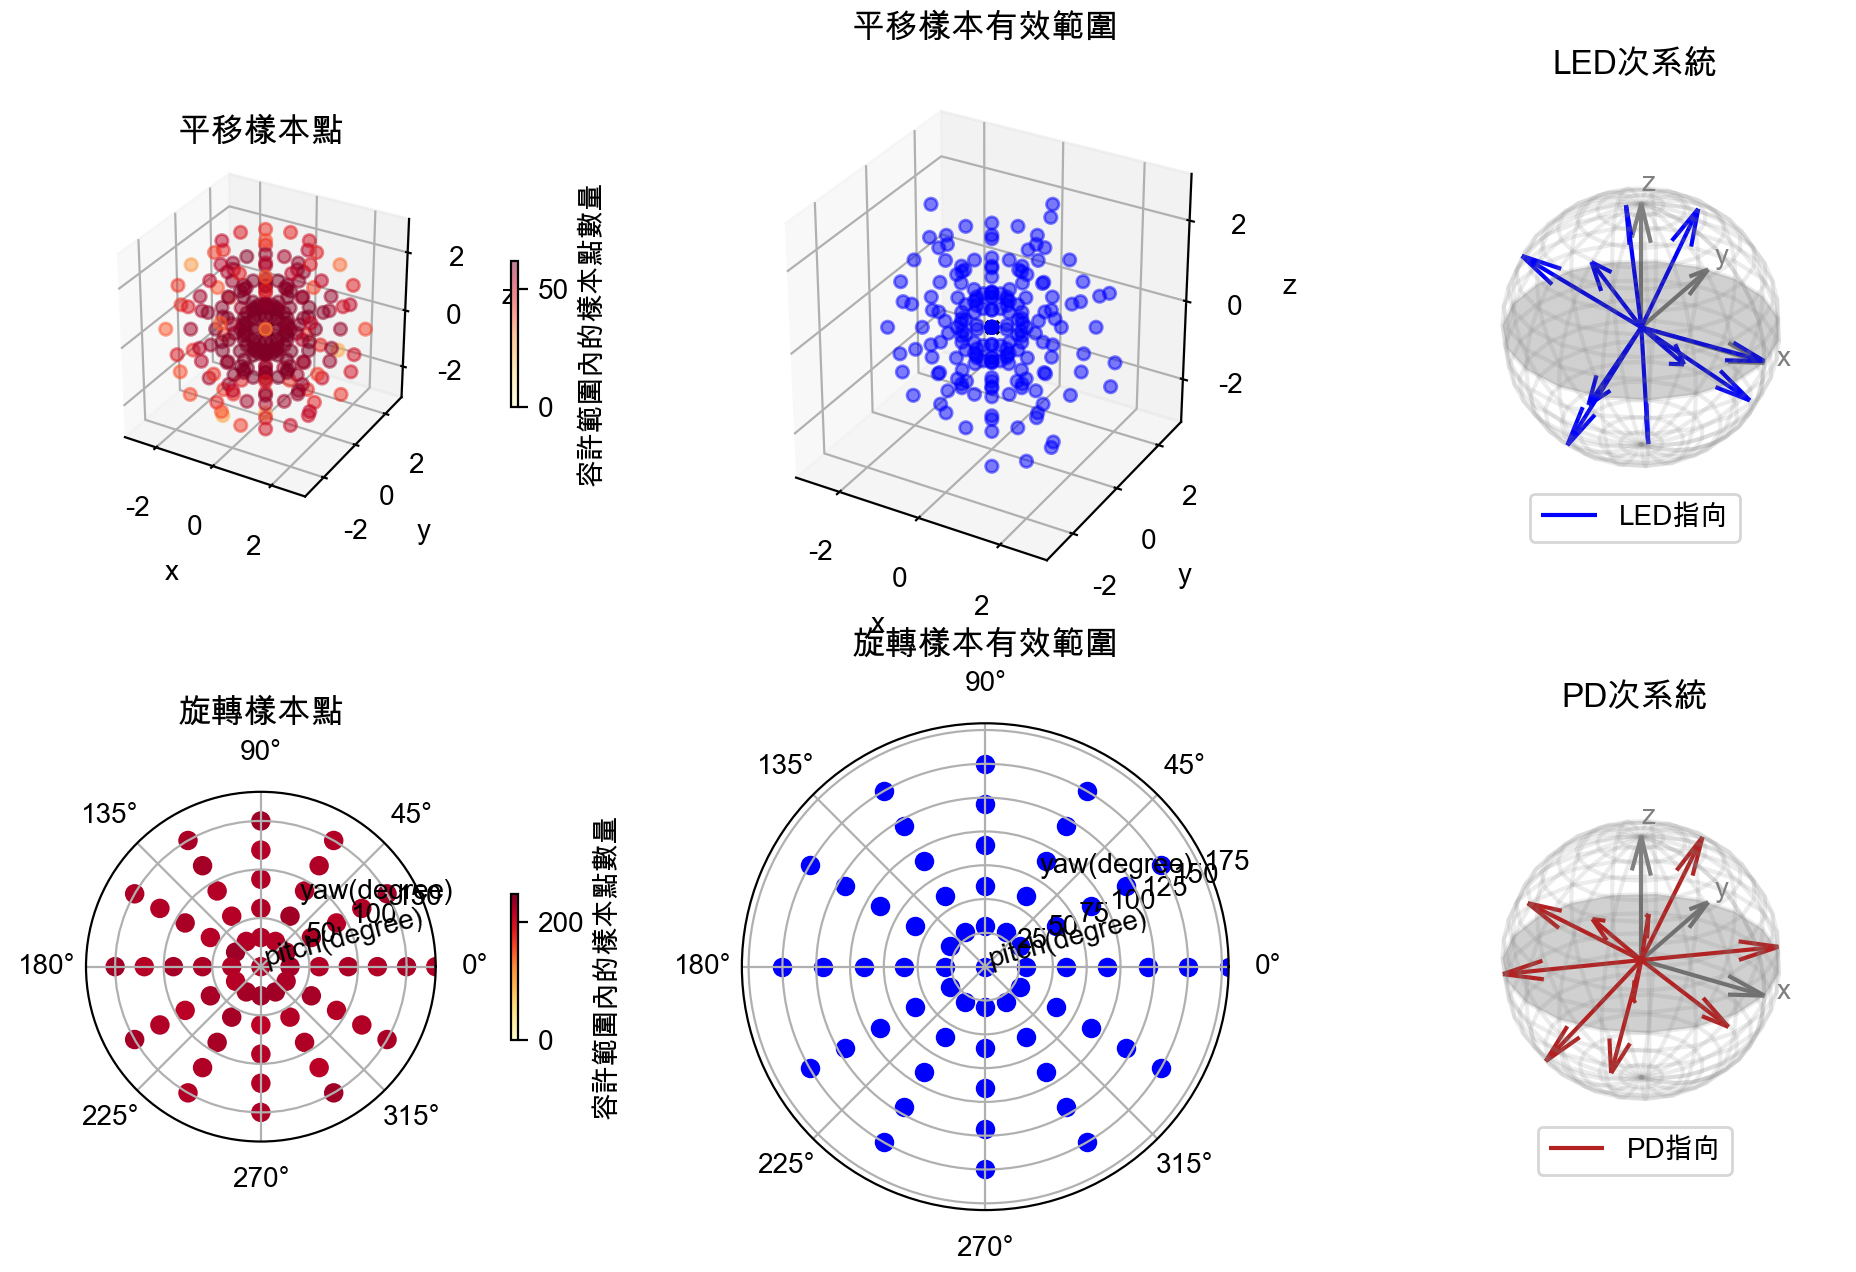
\includegraphics[width=15cm]{ch5pic/d_1010.png}
        \caption{情境甲於L=P=10的最佳系統表現與硬體擺設}
        \label{pic:d_1010}
    \end{figure}

    % \begin{table}[htpb]
    %     \begin{center}
    %       \caption{使用情境丁的最佳化結果}
    %       \label{tab:optimize_d}
    %       \begin{tabular}{c||c|c|c|c|c|cccccc} % <-- Alignments: 1st column left, 2nd middle and 3rd right, with vertical lines in between
    %         硬體數量$L=P$& 3&4&5&6&7&8&9&10&11&12&13\\
    %         \hline

    %         系統成效$Nt$&2149&2544&3439&4512&8571&13677&14151&14453&14534&14614&14624
    %       \end{tabular}
    %     \end{center}
    %   \end{table}

% --------------------------------------
% \subsection{小結}

% 由使用情境甲、丙、丁三個情境的最佳


\section{結論}
\label{chp:5_conclu}

本章節提出一流程,針對不同使用情境,設定一硬體數量$P,L$的設計空間,以進行朗博次方$Mp,M\ell$、硬體指向$^{P}\boldsymbol{V}_p,^{L}\boldsymbol{V}_l$共$2+2(L+P)$個變數的的最佳化。

% 透過設定不同的情境、不同的參數,我們可以得到最適合的朗博次方與硬體擺設設計,也知道不同硬體數量的表現。

本章節利用三個使用情境進行最佳化流程,其中使用情境甲中呈現出硬體數量與硬體擺設姿態的重要性,而由使用情境丙可以觀察到朗博次方對定位精度提升的效果,使用情境丁則是呈現一滿足本研究\ref{chp:motivate}章中兩硬體得以任意旋轉的使用情境。各使用情境的最佳化流程,僅能夠得到各硬體數量對應的硬體表現,而從中依照期待的系統成效和硬體系統成本、複雜度進行評估,選擇合適的硬體數量則是系統設計者的重要工作。

以實際應用層面來看,有了最佳化後的結果,我們可以參考最佳朗博次方,於市售硬體中挑選接近的硬體,並再以\ref{chp:simulation}章中介紹的模擬方式,對該次系統硬體規格的系統進行定位成效評估,確認次系統設計是否符合使用者對系統成效的需求,再進行硬體的購買,並根據最佳擺設方法進行硬體次系統的搭建。如此透過軟體的模擬與最佳化,我們可以減少硬體系統重複測試的麻煩,利用方便低成本的軟體模擬,在實際系統搭建前對該系統有理解,並得到最符合需求的次系統設計,同時也能夠透過第四章的分析了解調整不同參數與次系統設計對系統的影響,幫助對實際硬體校調。













